\chapter{Central Forces, Gravitation, and Celestial Mechanics}
\label{ch:central_forces}

\begin{chapterintro}
\textbf{Chapter Objectives:} In this chapter, we develop the complete analytical theory of central conservative forces. You will discover the fundamental consequences of angular momentum conservation and Kepler's law of areas; construct the one-dimensional effective radial potential $U_{\text{eff}}(r)$ with its centrifugal barrier; derive Binet's kinematic and dynamic formulas; solve the Kepler-Newton gravitational problem; prove Kepler's three laws; calculate interplanetary orbital transfers using the vis-viva equation; and analyze planetary gravitational assists and Rutherford scattering.
\end{chapterintro}

\section{Properties of Central Force Fields}

\begin{definitionbox}{Central Force Field}
A force field $\vec{F}(\vec{r})$ acting on a material point $M$ is said to be \textbf{central} with respect to a fixed origin $O$ if the line of action of the force passes through $O$ at every instant:
\begin{equation}
\vec{F}(\vec{r}) = F(r)\,\ur = F(r)\,\frac{\vec{r}}{r}, \qquad r = \norm{\vec{r}}.
\end{equation}
The force is said to be \textbf{attractive} if $F(r) < 0$ and \textbf{repulsive} if $F(r) > 0$.
\end{definitionbox}

\begin{figure}[htbp]
\centering
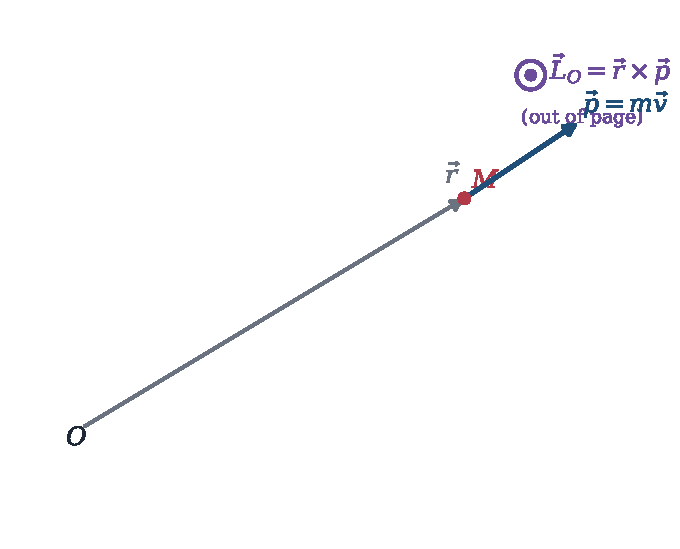
\includegraphics[width=0.74\textwidth]{figures/22_angular_momentum.pdf}
\caption{Conservation of angular momentum in central motion. The moment of a central force $\vec{F} = F(r)\ur$ with respect to center $O$ vanishes identically ($\vec{\mathcal{M}}_O = \vec{r}\times\vec{F} = \vzero$), freezing the angular momentum vector $\vec{L}_O = \vec{r}\times\vec{p}$ in magnitude and spatial orientation.}
\label{fig:angular_momentum}
\end{figure}

\begin{lawbox}{The Fundamental Theorem of Central Motion}
For any particle moving under a central force field centered at $O$, the angular momentum $\vec{L}_O$ with respect to $O$ is an invariant of motion:
\begin{equation}
\frac{\dd\vec{L}_O}{\dd t} = \vec{\mathcal{M}}_O(\vec{F}) = \vec{r} \times \vec{F} = \vec{r} \times (F(r)\ur) = \vzero \implies \vec{L}_O = \vec{r} \times m\vec{v} = \text{constant vector}.
\end{equation}
\textbf{Profound Geometrical Consequence (Planarity):}
Since $\vec{L}_O$ is a constant vector orthogonal to both $\vec{r}(t)$ and $\vec{v}(t)$ at every instant:
\begin{equation}
\vec{r}(t) \cdot \vec{L}_O \equiv 0.
\end{equation}
\textbf{The trajectory of a particle subject to a central force is strictly confined to a fixed two-dimensional plane} passing through the force center $O$ and perpendicular to $\vec{L}_O$.
\end{lawbox}

\section{Kepler's Second Law (Law of Areas) and Areal Velocity}

Adopting plane polar coordinates $(r, \theta)$ in the orbital plane with origin at $O$:
\[
\vec{r} = r\,\ur, \qquad \vec{v} = \dot{r}\,\ur + r\dot{\theta}\,\ut.
\]
The angular momentum vector is:
\begin{equation}
\vec{L}_O = \vec{r} \times m\vec{v} = (r\,\ur) \times m(\dot{r}\,\ur + r\dot{\theta}\,\ut) = m r^2 \dot{\theta}\,\khat \eqdef L\,\khat.
\end{equation}
Since $\vec{L}_O$ is constant, the scalar magnitude $L = m r^2 \dot{\theta}$ is strictly conserved:
\begin{equation}
C \eqdef r^2 \dot{\theta} = \frac{L}{m} = \text{constant of areas}.
\end{equation}

\begin{figure}[htbp]
\centering
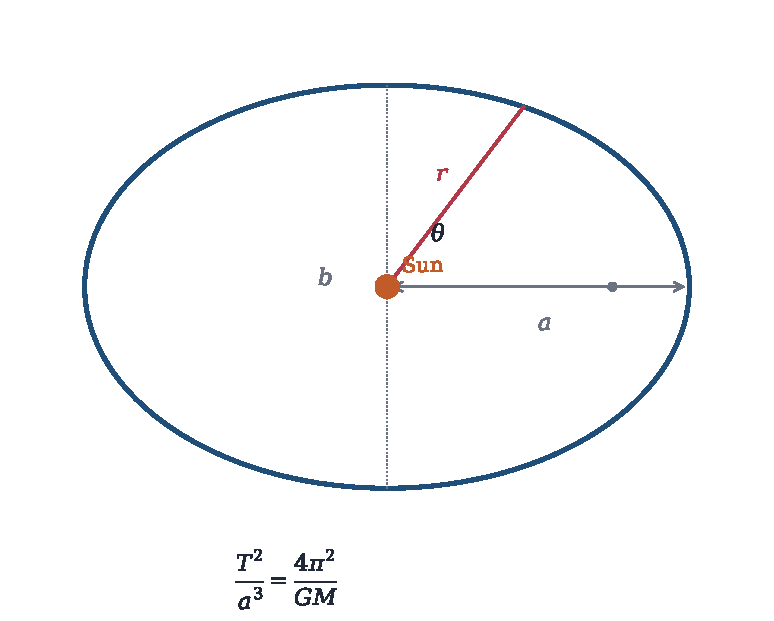
\includegraphics[width=0.74\textwidth]{figures/17_kepler.pdf}
\caption{Kepler's Second Law: equal areas in equal times. An orbiting body sweeps out equal planar sectors $\Delta A_1 = \Delta A_2$ in equal time intervals $\Delta t$, traveling fastest at perihelion ($r_{\min}$) and slowest at aphelion ($r_{\max}$).}
\label{fig:kepler}
\end{figure}

During an infinitesimal time $\dd t$, the position vector $\vec{r}$ rotates through angle $\dd\theta$, sweeping out an elementary triangular sector of area:
\begin{equation}
\dd A = \frac{1}{2} \norm{\vec{r} \times \dd\vec{r}} = \frac{1}{2} r (r\,\dd\theta) = \frac{1}{2} r^2 \dd\theta.
\end{equation}
Dividing by $\dd t$ yields the \textbf{areal velocity}:
\begin{equation}
\frac{\dd A}{\dd t} = \frac{1}{2} r^2 \dot{\theta} = \frac{C}{2} = \frac{L}{2m} = \text{constant}.
\end{equation}

\begin{lawbox}{Kepler's Second Law (Law of Areas)}
The radius vector joining the force center to the particle sweeps out equal planar areas in equal intervals of time throughout the entire motion:
\begin{equation}
\Delta A = \frac{L}{2m} \Delta t.
\end{equation}
As a direct consequence, the linear speed is inversely proportional to the instantaneous distance to the center: at perihelion ($r_p$), speed is maximum ($v_p = C/r_p$); at aphelion ($r_a$), speed is minimum ($v_a = C/r_a$).
\end{lawbox}

\begin{historicalbox}{Johannes Kepler and the New Astronomy}
\begin{minipage}{0.28\textwidth}
\centering
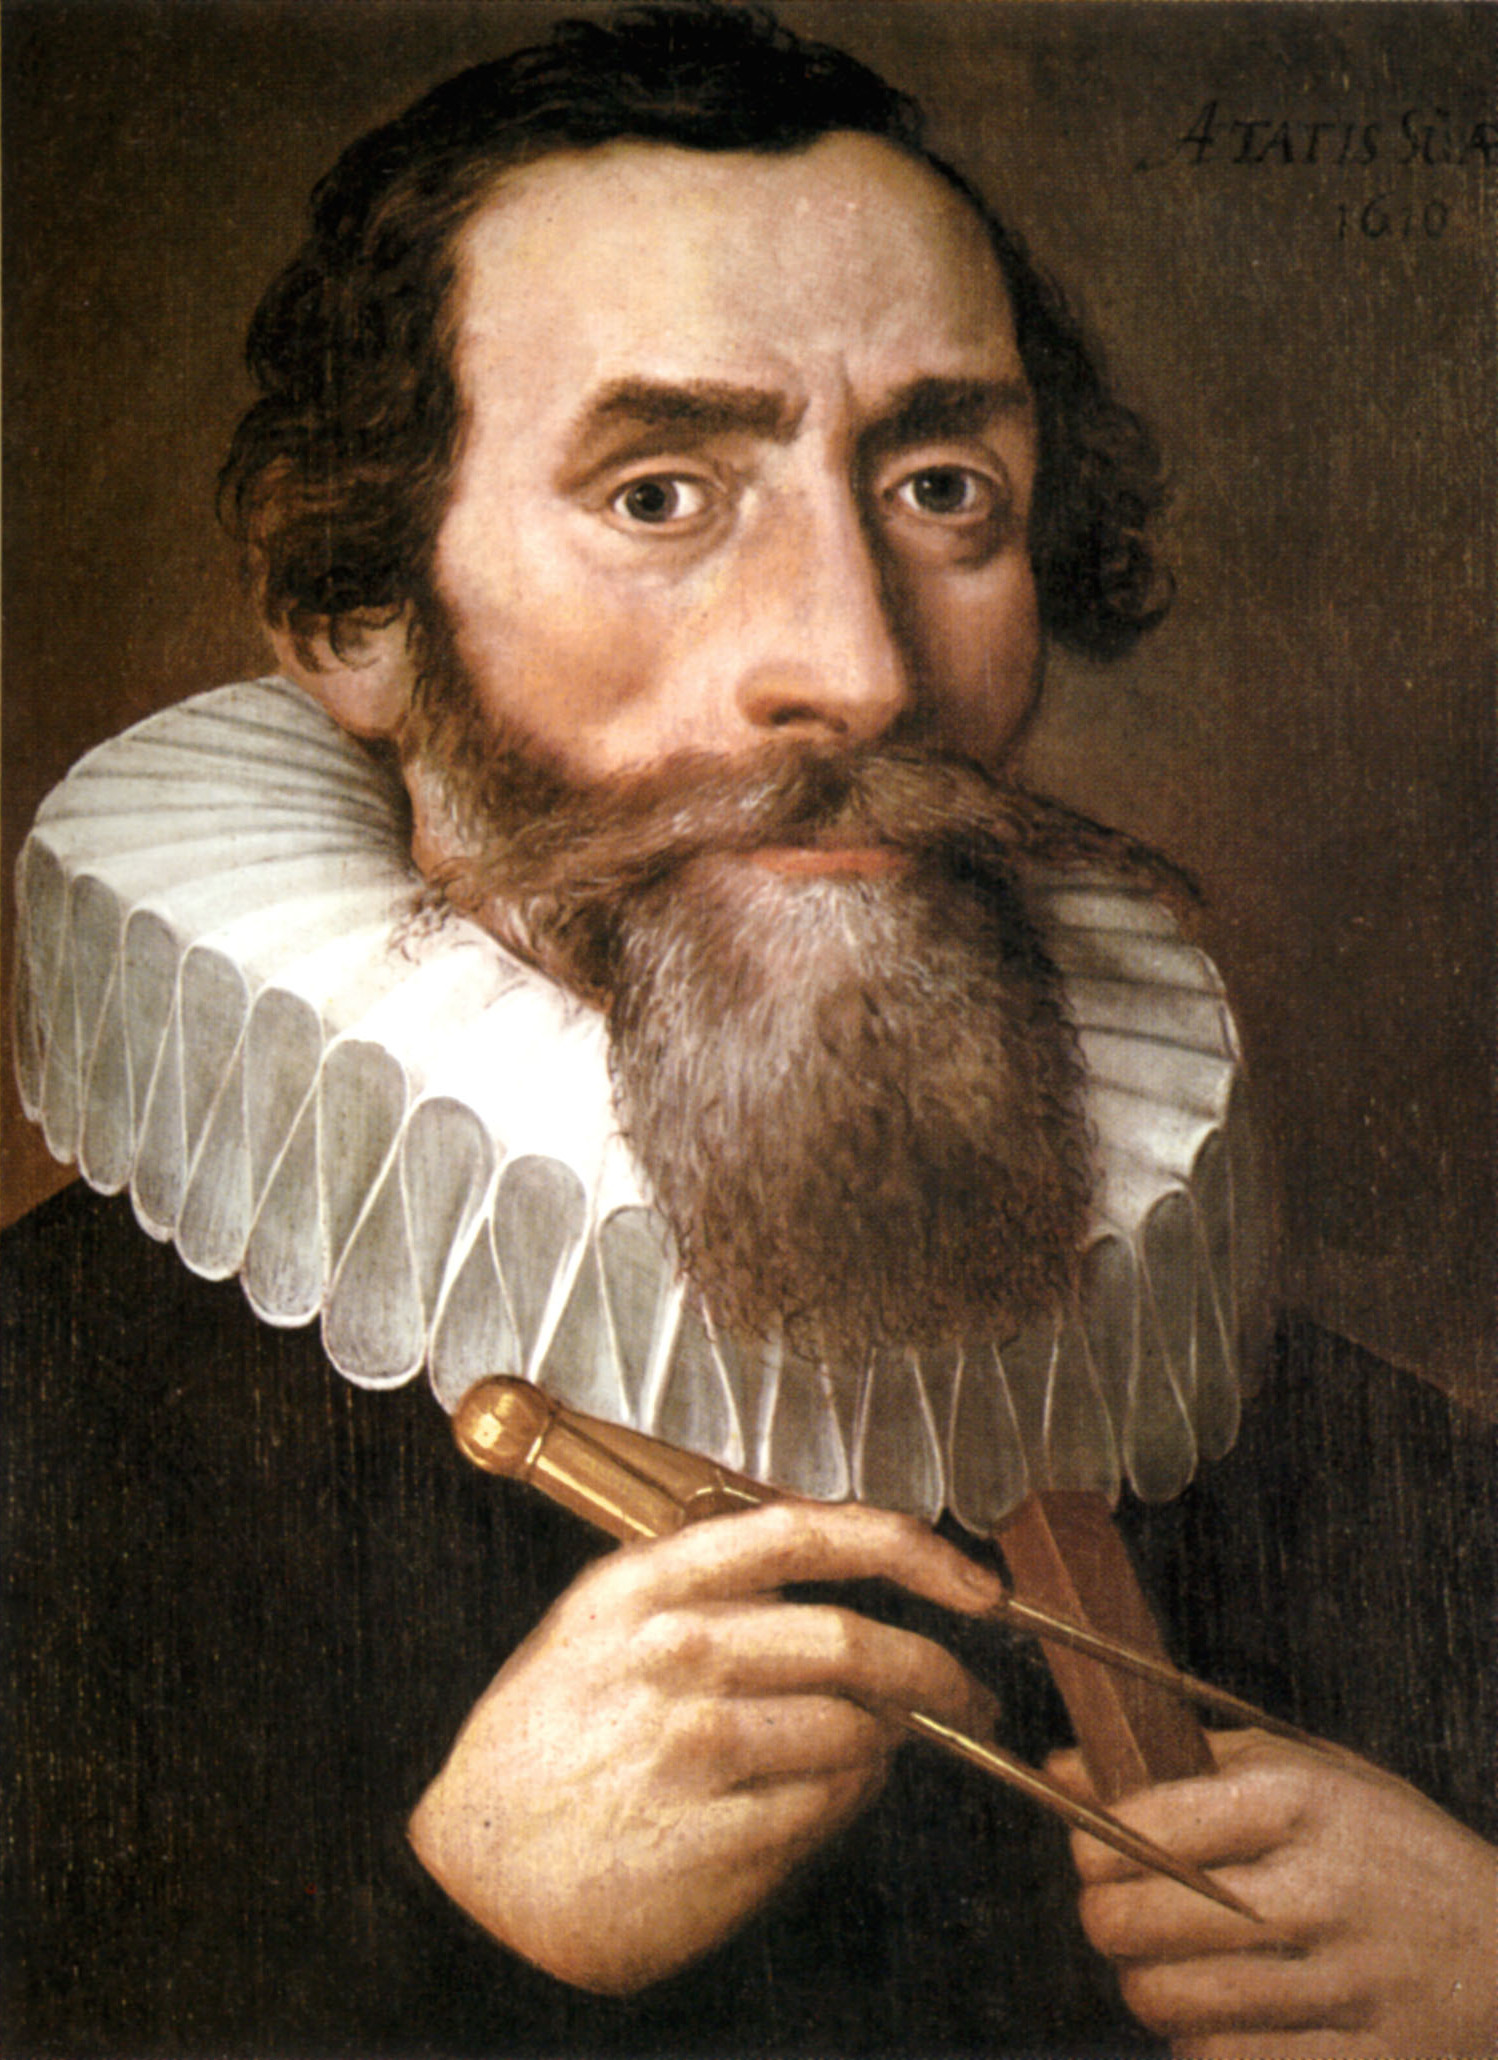
\includegraphics[width=0.92\textwidth]{images/kepler.jpg}
\captionof{figure}{Johannes Kepler (1571--1630), contemporary copper engraving (1610).}
\end{minipage}\hfill
\begin{minipage}{0.68\textwidth}
Working as imperial mathematician to Holy Roman Emperor Rudolf II in Prague, Johannes Kepler inherited decades of ultra-precise naked-eye planetary observations recorded by Tycho Brahe. 

Focusing on the stubborn 8-arcminute discrepancy in the orbit of Mars that could not be reconciled with circular epicycles, Kepler made the revolutionary conceptual leap in \emph{Astronomia Nova} (1609) that planetary orbits are not circles, but \textbf{ellipses with the Sun situated at one focus}. In \emph{Harmonices Mundi} (1619), he unveiled his Third Law, linking orbital periods to semi-major axes ($T^2 \propto a^3$), providing the decisive empirical foundation that led Isaac Newton to the inverse-square law of universal gravitation.
\end{minipage}
\end{historicalbox}

\section{The One-Dimensional Effective Radial Potential}

Because any central force is conservative ($\vec{\nabla}\times(F(r)\ur) = \vzero$), there exists a scalar potential $V(r)$ such that $F(r) = -\frac{\dd V}{\dd r}$.
The total mechanical energy in polar coordinates is:
\begin{equation}
E_m = \frac{1}{2}m v^2 + V(r) = \frac{1}{2}m(\dot{r}^2 + r^2\dot{\theta}^2) + V(r).
\end{equation}
Substituting $\dot{\theta} = \frac{L}{m r^2}$:
\begin{equation}
E_m = \frac{1}{2}m \dot{r}^2 + \frac{L^2}{2m r^2} + V(r) = \frac{1}{2}m \dot{r}^2 + U_{\text{eff}}(r).
\end{equation}

\begin{definitionbox}{Effective Potential Energy}
The two-dimensional central motion is mathematically equivalent to the one-dimensional motion of a fictitious particle of mass $m$ moving in the \textbf{effective radial potential}:
\begin{equation}
U_{\text{eff}}(r) \eqdef V(r) + \frac{L^2}{2m r^2}.
\end{equation}
The term $\frac{L^2}{2m r^2} > 0$ is the \textbf{centrifugal potential barrier}, which acts as a repulsive core preventing any particle with non-zero angular momentum ($L \neq 0$) from collapsing into the origin.
\end{definitionbox}

\section{Binet's Formulas for Trajectory Calculation}

Jacques Philippe Marie Binet (1835) introduced the reciprocal radial variable:
\begin{equation}
u(\theta) \eqdef \frac{1}{r(\theta)}.
\end{equation}
Using the chain rule $\frac{\dd}{\dd t} = \dot{\theta} \frac{\dd}{\dd\theta} = C u^2 \frac{\dd}{\dd\theta}$, the radial position is $r = 1/u$, and the radial velocity is:
\begin{equation}
\dot{r} = \frac{\dd}{\dd t}\left(\frac{1}{u}\right) = -\frac{1}{u^2}\dot{u} = -\frac{1}{u^2} (C u^2) \frac{\dd u}{\dd\theta} = -C \frac{\dd u}{\dd\theta}.
\end{equation}

\begin{lawbox}{Binet's Formulas}
\begin{enumerate}[leftmargin=1.5em,itemsep=3pt]
  \item \textbf{Binet's Kinematic Velocity Formula:}
  \begin{equation}
  v^2 = \dot{r}^2 + r^2\dot{\theta}^2 = C^2 \left[ u^2 + \left(\frac{\dd u}{\dd\theta}\right)^2 \right].
  \end{equation}
  \item \textbf{Binet's Dynamic Acceleration Formula:}
  Differentiating $\dot{r}$ with respect to time and computing radial acceleration $a_r = \ddot{r} - r\dot{\theta}^2$:
  \begin{equation}
  a_r = -C^2 u^2 \left( \frac{\dd^2 u}{\dd\theta^2} + u \right) = \frac{F(1/u)}{m}.
  \end{equation}
\end{enumerate}
\end{lawbox}

\section{The Kepler-Newton Gravitational Problem}

For Newtonian gravitation, the interaction between a central mass $M$ and a satellite mass $m \ll M$ is:
\begin{equation}
\vec{F} = -\frac{G M m}{r^2}\,\ur = -k u^2\,\ur, \qquad k \eqdef G M m.
\end{equation}
Substituting $F(1/u) = -k u^2$ into Binet's dynamic equation:
\[
-C^2 u^2 \left( \frac{\dd^2 u}{\dd\theta^2} + u \right) = -\frac{k u^2}{m} \implies \frac{\dd^2 u}{\dd\theta^2} + u = \frac{k}{m C^2}.
\]
Defining the geometric parameter $p \eqdef \frac{m C^2}{k} = \frac{L^2}{m k}$, known as the \textbf{semi-latus rectum}:
\begin{equation}
\frac{\dd^2 u}{\dd\theta^2} + u = \frac{1}{p}.
\end{equation}
This is the elementary harmonic oscillator differential equation shifted by the constant $1/p$. Its general solution is:
\begin{equation}
u(\theta) = \frac{1}{p}\left[ 1 + e \cos(\theta - \theta_0) \right].
\end{equation}
Choosing the polar axis $\theta = 0$ at periapsis ($\theta_0 = 0$):

\begin{lawbox}{The Conic Equation of Keplerian Orbits}
The trajectory $r(\theta) = 1/u(\theta)$ is a conic section with the gravitational center at one focus:
\begin{equation}
r(\theta) = \frac{p}{1 + e \cos\theta},
\end{equation}
where $e \ge 0$ is the orbital \textbf{eccentricity}, uniquely determined by the mechanical energy $E_m$ and angular momentum $L$:
\begin{equation}
e = \sqrt{1 + \frac{2 E_m L^2}{m k^2}} = \sqrt{1 + \frac{2 E_m C^2 m}{k^2}}.
\end{equation}
\end{lawbox}

\begin{table}[htbp]
\centering
\renewcommand{\arraystretch}{1.35}
\begin{tabular}{@{}llll@{}}
\toprule
\textbf{Energy $E_m$} & \textbf{Eccentricity $e$} & \textbf{Conic Geometry} & \textbf{Physical State} \\
\midrule
$E_m = E_{\min} = -\frac{m k^2}{2 L^2}$ & $e = 0$ & Circle ($r = p = \text{const}$) & Bound periodic orbit \\
$E_{\min} < E_m < 0$ & $0 < e < 1$ & Ellipse ($a = \frac{p}{1-e^2}$) & Bound periodic orbit (Planets, Moons) \\
$E_m = 0$ & $e = 1$ & Parabola ($r_p = p/2$) & Marginally escape threshold \\
$E_m > 0$ & $e > 1$ & Hyperbola ($a = \frac{p}{e^2-1}$) & Unbound flyby trajectory (Comets, Oumuamua) \\
\bottomrule
\end{tabular}
\caption{Classification of Keplerian conic trajectories by energy and eccentricity.}
\label{tab:kepler_conics}
\end{table}

\subsection{Kepler's Third Law and the Vis-Viva Equation}

For an elliptical orbit of semi-major axis $a$ and semi-minor axis $b = a\sqrt{1-e^2}$:
\begin{itemize}[leftmargin=1.5em,itemsep=3pt]
  \item The total orbital area is $A = \pi a b$.
  \item By the law of areas, $\Delta A = \frac{C}{2} T \implies \pi a b = \frac{C}{2} T$.
  \item Since $p = a(1-e^2) = \frac{b^2}{a}$ and $p = \frac{m C^2}{k} = \frac{C^2}{G M}$:
  \[
  C = \sqrt{G M p} = \sqrt{G M \frac{b^2}{a}} = \frac{b}{\sqrt{a}}\sqrt{G M}.
  \]
  \item Squaring the period relation:
  \begin{equation}
  T^2 = \frac{4\pi^2 a^2 b^2}{C^2} = \frac{4\pi^2 a^2 b^2}{(b^2/a) G M} \implies \frac{T^2}{a^3} = \frac{4\pi^2}{G M}.
  \end{equation}
\end{itemize}

\begin{lawbox}{Kepler's Third Law}
The square of the orbital period $T$ of a planet is directly proportional to the cube of the semi-major axis $a$ of its elliptical orbit:
\begin{equation}
\frac{T^2}{a^3} = \frac{4\pi^2}{G(M + m)} \approx \frac{4\pi^2}{G M_\odot}.
\end{equation}
\end{lawbox}

\begin{lawbox}{The Vis-Viva Equation}
For any Keplerian orbit around a central mass $M$, the speed $v(r)$ at distance $r$ is:
\begin{equation}
v^2(r) = G M \left( \frac{2}{r} - \frac{1}{a} \right),
\end{equation}
where $a > 0$ for an ellipse, $a \to \infty$ for a parabola ($v^2 = 2GM/r$), and $a < 0$ for a hyperbola.
\end{lawbox}

\section{Comprehensive Worked Examples}

\begin{workedexample}{The Hohmann Interplanetary Transfer Orbit}
A robotic spacecraft in a circular Low Earth Parking Orbit (LEO) of radius $r_1 = 1.000\ \mathrm{AU} = 1.496\times 10^{11}\ \mathrm{m}$ is to be sent to Mars, whose orbit is modeled as circular and coplanar with radius $r_2 = 1.524\ \mathrm{AU} = 2.280\times 10^{11}\ \mathrm{m}$. Heliocentric gravitation is $G M_\odot = 1.327\times 10^{20}\ \mathrm{m^3\cdot s^{-2}}$.
\begin{enumerate}[leftmargin=1.4em,itemsep=3pt]
  \item Calculate the semi-major axis $a_t$ and the flight duration $\Delta t_{\text{trans}}$ of the elliptical Hohmann transfer orbit.
  \item Compute the orbital speeds $v_1$ (Earth) and $v_2$ (Mars), and determine the injection burn velocity increment $\Delta v_1$ required at perihelion.
  \item Determine the arrival velocity increment $\Delta v_2$ required at aphelion to circularize into Mars's orbit.
\end{enumerate}

\paragraph{Solution.}
\textbf{1. Semi-Major Axis and Transfer Time:}\\
The Hohmann transfer orbit is an ellipse whose perihelion is at Earth ($r_p = r_1$) and whose aphelion is at Mars ($r_a = r_2$). The major axis is the sum:
\[
2a_t = r_1 + r_2 \implies a_t = \frac{r_1 + r_2}{2} = \frac{1.000 + 1.524}{2} = 1.262\ \mathrm{AU} = 1.888\times 10^{11}\ \mathrm{m}.
\]
By Kepler's Third Law, the period of the full transfer ellipse is:
\[
T_t = 1\ \mathrm{yr} \times \left(\frac{a_t}{1\ \mathrm{AU}}\right)^{3/2} = (1.262)^{3/2} \approx 1.4177\ \mathrm{years} \approx 517.8\ \mathrm{days}.
\]
Because the spacecraft traverses exactly half of the ellipse (from perihelion to aphelion), the one-way transit time is:
\[
\Delta t_{\text{trans}} = \frac{1}{2} T_t = \frac{517.8}{2} \approx 258.9\ \mathrm{days} \approx 8.5\ \mathrm{months}.
\]

\textbf{2. Heliocentric Speeds and Injection Burn $\Delta v_1$:}\\
Earth's circular orbital speed is:
\[
v_1 = \sqrt{\frac{G M_\odot}{r_1}} = \sqrt{\frac{1.327\times 10^{20}}{1.496\times 10^{11}}} \approx 29\,780\ \mathrm{m\cdot s^{-1}} \approx 29.78\ \mathrm{km\cdot s^{-1}}.
\]
Mars's circular orbital speed is:
\[
v_2 = \sqrt{\frac{G M_\odot}{r_2}} = \sqrt{\frac{1.327\times 10^{20}}{2.280\times 10^{11}}} \approx 24\,120\ \mathrm{m\cdot s^{-1}} \approx 24.12\ \mathrm{km\cdot s^{-1}}.
\]
Using the vis-viva equation $v^2 = G M_\odot(2/r - 1/a)$, the speed on the transfer ellipse at perihelion ($r = r_1$) is:
\[
v_{t,1} = \sqrt{G M_\odot\left(\frac{2}{r_1} - \frac{1}{a_t}\right)} = \sqrt{1.327\times 10^{20}\left( \frac{2}{1.496\times 10^{11}} - \frac{1}{1.888\times 10^{11}} \right)}.
\]
\[
v_{t,1} = \sqrt{1.327\times 10^{20}(1.3369\times 10^{-11} - 0.5297\times 10^{-11})} = \sqrt{1.071\times 10^9} \approx 32\,730\ \mathrm{m\cdot s^{-1}} \approx 32.73\ \mathrm{km\cdot s^{-1}}.
\]
The required injection boost relative to Earth's heliocentric velocity is:
\[
\Delta v_1 = v_{t,1} - v_1 = 32.73 - 29.78 = 2.95\ \mathrm{km\cdot s^{-1}}.
\]

\textbf{3. Arrival Burn $\Delta v_2$ at Mars:}\\
The speed on the transfer ellipse at aphelion ($r = r_2$) is:
\[
v_{t,2} = \sqrt{G M_\odot\left(\frac{2}{r_2} - \frac{1}{a_t}\right)} = \sqrt{1.327\times 10^{20}\left( \frac{2}{2.280\times 10^{11}} - \frac{1}{1.888\times 10^{11}} \right)}.
\]
\[
v_{t,2} = \sqrt{1.327\times 10^{20}(0.8772\times 10^{-11} - 0.5297\times 10^{-11})} = \sqrt{4.611\times 10^8} \approx 21\,470\ \mathrm{m\cdot s^{-1}} \approx 21.47\ \mathrm{km\cdot s^{-1}}.
\]
To match Mars's circular speed $v_2 = 24.12\ \mathrm{km/s}$, the spacecraft must fire thrusters forward to gain speed:
\[
\Delta v_2 = v_2 - v_{t,2} = 24.12 - 21.47 = 2.65\ \mathrm{km\cdot s^{-1}}.
\]
The total mission delta-v budget is $\Delta v_{\text{total}} = \Delta v_1 + \Delta v_2 = 2.95 + 2.65 = 5.60\ \mathrm{km\cdot s^{-1}}$.
\end{workedexample}

\begin{workedexample}{Planetary Gravity Assist (The Gravitational Slingshot)}
A scientific space probe of mass $m$ encounters Jupiter (mass $M_J \gg m$) on an interplanetary trajectory. In the heliocentric frame $\mathcal{R}_{\odot}$, Jupiter moves with orbital velocity $\vec{V}_J = V_J\,\jhat$ ($V_J \approx 13.0\ \mathrm{km\cdot s^{-1}}$). The probe approaches Jupiter along the $-\jhat$ direction with asymptotic speed $v_0 = 10.0\ \mathrm{km\cdot s^{-1}}$, so $\vec{v}_{\text{in}} = -v_0\,\jhat$.
\begin{enumerate}[leftmargin=1.4em,itemsep=3pt]
  \item Determine the approach speed $u_\infty$ in the rest frame of Jupiter $\mathcal{R}_J$.
  \item The hyperbolic trajectory swings around Jupiter such that its exit velocity is turned by an angle $\delta = 180^\circ$ (a head-on retrograde slingshot). Compute the final heliocentric velocity $\vec{v}_{\text{out}}$ and the kinetic energy gained by the probe.
  \item Explain the source of the mechanical energy gained by the probe.
\end{enumerate}

\paragraph{Solution.}
\textbf{1. Approach Velocity in Jupiter's Rest Frame:}\\
Using the Galilean velocity transformation $\vec{u} = \vec{v} - \vec{V}_J$:
\[
\vec{u}_{\text{in}} = \vec{v}_{\text{in}} - \vec{V}_J = -v_0\,\jhat - V_J\,\jhat = -(v_0 + V_J)\,\jhat.
\]
The relative entry speed is $u_\infty = v_0 + V_J = 10.0 + 13.0 = 23.0\ \mathrm{km\cdot s^{-1}}$.

\textbf{2. Slingshot Acceleration in Heliocentric Frame:}\\
In Jupiter's frame $\mathcal{R}_J$, the gravitational interaction is purely conservative. Because the probe enters and exits from essentially infinite distance ($r \to \infty$ where $V(r) \to 0$), energy conservation dictates:
\[
\frac{1}{2}m u_{\text{out}}^2 = \frac{1}{2}m u_{\text{in}}^2 \implies u_{\text{out}} = u_{\text{in}} = u_\infty.
\]
The planet merely \textbf{rotates} the velocity vector without changing its magnitude in its own frame!
For a maximum deflection angle $\delta = 180^\circ$, the probe exits directed along $+\jhat$:
\[
\vec{u}_{\text{out}} = +u_\infty\,\jhat = +(v_0 + V_J)\,\jhat.
\]
Transforming back to the heliocentric frame $\mathcal{R}_\odot$:
\[
\vec{v}_{\text{out}} = \vec{u}_{\text{out}} + \vec{V}_J = +(v_0 + V_J)\,\jhat + V_J\,\jhat = (v_0 + 2V_J)\,\jhat.
\]
Plugging in the numerical values:
\[
v_{\text{out}} = 10.0 + 2(13.0) = 36.0\ \mathrm{km\cdot s^{-1}}!
\]
The heliocentric speed increased dramatically from $10.0\ \mathrm{km/s}$ to $36.0\ \mathrm{km/s}$ ($\Delta v = +26.0\ \mathrm{km/s} = 2V_J$).
The kinetic energy of the probe increased by:
\[
\Delta E_k = \frac{1}{2}m v_{\text{out}}^2 - \frac{1}{2}m v_{\text{in}}^2 = \frac{1}{2}m \left( 36^2 - 10^2 \right) = \frac{1}{2}m(1296 - 100) = 598\,m\ \mathrm{MJ\cdot kg^{-1}}.
\]

\textbf{3. Source of the Gained Energy:}\\
Total energy and linear momentum of the combined probe-Jupiter system are strictly conserved in the heliocentric frame. The enormous kinetic energy gained by the spacecraft is extracted directly from the \textbf{orbital kinetic energy of Jupiter}:
\[
\Delta E_J = -\Delta E_{\text{probe}} = -598\,m.
\]
Because $M_J \approx 1.90\times 10^{27}\ \mathrm{kg}$, for a probe of $m = 1000\ \mathrm{kg}$, Jupiter's orbital speed slows down by:
\[
\Delta V_J \approx -\frac{m}{M_J} \Delta v \approx -\frac{10^3}{1.9\times 10^{27}}(2.6\times 10^4) \approx -1.4\times 10^{-20}\ \mathrm{m\cdot s^{-1}},
\]
an imperceptible slowing of Jupiter that permanently boosted Voyager 1 and 2 onto hyperbolic escape trajectories from the Solar System!
\end{workedexample}

\begin{workedexample}{Rutherford Alpha Particle Scattering Formula}
An alpha particle (charge $q_1 = +2e$, mass $m_\alpha$) approaches a heavy gold nucleus (charge $q_2 = +Ze$, mass $M \gg m_\alpha$) with initial impact parameter $b$ and asymptotic speed $v_0$. The repulsive Coulomb potential is:
\begin{equation}
V(r) = \frac{1}{4\pi\varepsilon_0}\frac{2Ze^2}{r} = \frac{k_c}{r}, \qquad k_c \eqdef \frac{2Ze^2}{4\pi\varepsilon_0}.
\end{equation}
\begin{enumerate}[leftmargin=1.4em,itemsep=3pt]
  \item Using angular momentum $L = m_\alpha v_0 b$ and Binet's equation, show that the trajectory is a hyperbola of the form $u(\theta) = \frac{1}{p}(e\cos\theta - 1)$.
  \item Establish the exact relation between the impact parameter $b$ and the scattering deflection angle $\theta_s$:
  \begin{equation}
  b = \frac{k_c}{2 E_k} \cot\left(\frac{\theta_s}{2}\right), \qquad E_k = \frac{1}{2}m_\alpha v_0^2.
  \end{equation}
  \item Compute the distance of closest approach $r_{\min}$ for a direct head-on collision ($b = 0$, $\theta_s = 180^\circ$).
\end{enumerate}

\paragraph{Solution.}
\textbf{1. Hyperbolic Trajectory via Binet's Equation:}\\
The Coulomb force is repulsive: $\vec{F} = +\frac{k_c}{r^2}\ur = +k_c u^2\ur$. Binet's dynamic formula gives:
\[
-C^2 u^2\left(\frac{\dd^2 u}{\dd\theta^2} + u\right) = \frac{k_c u^2}{m_\alpha} \implies \frac{\dd^2 u}{\dd\theta^2} + u = -\frac{k_c}{m_\alpha C^2} \eqdef -\frac{1}{p},
\]
where $p = \frac{m_\alpha C^2}{k_c} = \frac{L^2}{m_\alpha k_c} = \frac{m_\alpha v_0^2 b^2}{k_c}$.
The general solution symmetric about the periapsis axis $\theta = 0$ is:
\[
u(\theta) = \frac{1}{p}(e\cos\theta - 1) \implies r(\theta) = \frac{p}{e\cos\theta - 1}.
\]
Because $r > 0$ physically, the motion is bounded to angular sectors where $e\cos\theta > 1$. The asymptotic directions $r \to \infty$ ($u \to 0$) satisfy:
\[
e\cos\theta_\infty - 1 = 0 \implies \cos\theta_\infty = \frac{1}{e}.
\]

\textbf{2. Relation Between Impact Parameter $b$ and Deflection Angle $\theta_s$:}\\
The incoming asymptote is at angle $-\theta_\infty$, and the outgoing asymptote is at $+\theta_\infty$.
The scattering angle $\theta_s$ by which the trajectory is deflected from its initial straight line is:
\[
\theta_s = \pi - 2\theta_\infty \implies \frac{\theta_s}{2} = \frac{\pi}{2} - \theta_\infty \implies \sin\left(\frac{\theta_s}{2}\right) = \cos\theta_\infty = \frac{1}{e}.
\]
Thus:
\[
\cot\left(\frac{\theta_s}{2}\right) = \frac{\cos(\theta_s/2)}{\sin(\theta_s/2)} = \frac{\sqrt{1 - 1/e^2}}{1/e} = \sqrt{e^2 - 1}.
\]
Squaring this relation:
\[
e^2 - 1 = \cot^2\left(\frac{\theta_s}{2}\right).
\]
From the energy relation for the Coulomb potential, $E_m = E_k = \frac{1}{2}m_\alpha v_0^2 > 0$:
\[
e = \sqrt{1 + \frac{2 E_m L^2}{m_\alpha k_c^2}} \implies e^2 - 1 = \frac{2 E_k (m_\alpha v_0 b)^2}{m_\alpha k_c^2} = \frac{2 E_k (2 E_k) b^2}{k_c^2} = \left(\frac{2 E_k b}{k_c}\right)^2.
\]
Taking the square root:
\[
\frac{2 E_k b}{k_c} = \cot\left(\frac{\theta_s}{2}\right) \implies b = \frac{k_c}{2 E_k} \cot\left(\frac{\theta_s}{2}\right).
\]

\textbf{3. Head-On Collision Distance of Closest Approach:}\\
For a head-on collision ($b = 0$), the deflection is $\theta_s = 180^\circ$. At the point of closest approach $r_{\min}$, all kinetic energy is converted into Coulomb potential energy:
\[
E_k = \frac{k_c}{r_{\min}} \implies r_{\min} = \frac{k_c}{E_k} = \frac{2Ze^2}{4\pi\varepsilon_0 \left(\frac{1}{2}m_\alpha v_0^2\right)}.
\]
For a $5.0\ \mathrm{MeV}$ alpha particle scattered by a gold nucleus ($Z = 79$):
\[
r_{\min} = \frac{2(79)(1.44\ \mathrm{MeV\cdot fm})}{5.0\ \mathrm{MeV}} \approx 45.5\ \mathrm{fm} = 4.55\times 10^{-14}\ \mathrm{m}.
\]
Because $r_{\min}$ was orders of magnitude smaller than the Thomson atomic radius ($10^{-10}\ \mathrm{m}$), Ernest Rutherford deduced in 1911 that the positive charge and mass of the atom are concentrated in a tiny dense nucleus.
\end{workedexample}
